\chapter{Marco Teórico}\label{cap:marco_teorico}
En la última década, el desarrollo de software ha evolucionado en la dirección del \textbf{Continuous Software Engineering (CSE)}, que tiene como objetivo establecer un movimiento continuo en las actividades de la ingeniería de software, en lugar de un conjunto de actividades discretas realizadas por diferentes equipos o departamentos \cite{FITZGERALD2017176}.

Para permitir este movimiento continuo, CSE agrupa un conjunto de prácticas continuas como \textbf{Continuous Integration (CI)}. En la industria, las prácticas continuas relacionadas con el desarrollo cada vez se utilizan con mayor frecuencia y ya están bien establecidas \cite{Bosch2014}. Gran parte de la investigación sobre prácticas continuas se ha realizado sobre prácticas relacionadas con el desarrollo  \cite{Shahin2017ContinuousID}, \cite{10.1007/s10664-018-9651-4}, \cite{Schermann}, \cite{10.1145/3383219.3383224}. Según estos estudios, \textbf{Continuous Integration (CI)}, \textbf{Continuous Delivery (CDE)} y \textbf{Continuous Deployment (CD)} pueden verse como las prácticas continuas más populares en el dominio de CSE \cite{Sthl2017ContinuousPA}. Hemos seleccionado estas tres prácticas para su revisión en nuestra propuesta de \textbf{Práctica Supervisada (PS)}.

\textbf{Continuous Integration (CI)} es la práctica de desarrollo de software donde los miembros integran con frecuencia su trabajo (p. ej., cambios de código) en la rama principal, normalmente a diario \cite{Sthl2017ContinuousPA}.  Estos cambios son validados por compilaciones y pruebas automatizadas \cite{7057604}. Al hacerlo, los desarrolladores pueden detectar y abordar fallas de integración de manera temprana y lo más rápido posible \cite{7057604}, \cite{FITZGERALD2017176}.

\textbf{Continuous Delivery (CDE)} tiene como objetivo mantener el software en un estado de implementación confiable o listo para producción en todo momento \cite{10.1007/s10664-018-9651-4}, \cite{7006384}. Para lograr este objetivo, el software debe pasar pruebas y controles de calidad pertinentes en un entorno de prueba (p. ej., pruebas de aceptación). Sin embargo, la implementación en el entorno de producción se realiza de forma manual, donde un miembro del equipo con la autoridad pertinente decide cuándo y qué resultados listos para la producción se deben entregar al cliente (es decir, enfoque basado en extracción) \cite{10.1007/s10664-018-9651-4}.

\textbf{Continuous Deployment (CD)} Tiene como objetivo ampliar CDE mediante la implementación automática y continua de despliegues de software en un entorno de producción. Se supone que se han superado todos los objetivos de calidad requeridos \cite{7465693}, \cite{Shahin2017ContinuousID}. CD es un enfoque basado en “push”, donde los cambios de software se implementan directamente sobre producción a través del “pipeline” de implementación sin intervención humana \cite{Schermann}. 

En la Figura \ref{fig:pipeline1} se muestra la relación entre estas prácticas continuas, que se va a considerar en esta Práctica Supervisada.

\begin{figure}[htp]
    \centering
    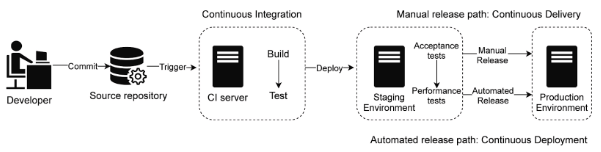
\includegraphics[width=0.9\textwidth]{fig/pipeline1.png}
    \caption{Relaciones entre las prácticas continuas CI, CDE y CD.}
    \label{fig:pipeline1}
\end{figure}
\textbf{DevOps}, una combinación de los términos desarrollo (development) y operaciones (operations), es un enfoque de trabajo que tiene como finalidad  minimizar la desconexión entre los equipos de desarrollo y operaciones mediante la promoción de la colaboración, comunicación y la integración entre ellos \cite{BassDevOpsA2015}. A pesar de ser una tendencia en la industria, DevOps carece de una definición ampliamente aceptada \cite{10.1145/3359981}. Definir DevOps es difícil debido a la considerable superposición con las prácticas continuas \cite{Sthl2017ContinuousPA}. Por esta razón, Stahl et al. \cite{Sthl2017ContinuousPA} presentan definiciones para diferenciar DevOps y prácticas continuas entre sí. En el presente trabajo se considera DevOps compuesto por las prácticas continuas antes mencionadas.

\textbf{DevOps} permite eliminar la barrera que había en una empresa u organización entre los desarrolladores  y  los encargados de las operaciones, permitiendo que se coordinen y colaboren para obtener productos mejores y más confiables. Al adoptar una cultura de DevOps junto a prácticas y herramientas, los equipos adquieren por un lado la  capacidad de responder mejor a las necesidades de los clientes y aumentar la confianza en las aplicaciones que crean y por otro lado alcanzar los objetivos empresariales en menos tiempo. Se emplea el término \textbf{Pipeline} para referirnos al flujo de trabajo y a las tareas a realizar en todas las etapas del desarrollo de software. En la Figura \ref{fig:pipeline2} se ilustran las etapas que componen al pipeline de DevOps.

\begin{figure}[H]
    \centering
    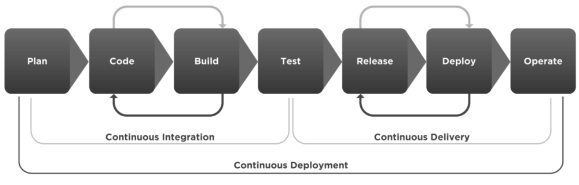
\includegraphics[width=0.9\textwidth]{fig/pipeline2.png}
    \caption{Etapas del Pipeline DevOps.}
    \label{fig:pipeline2}
\end{figure}

Esta nueva forma de trabajar se puede aplicar a los sistemas ciber físicos \textbf{(Cyber Physical Systems, CPS)}, en los cuales se integra la computación, almacenamiento y comunicación junto con capacidades de seguimiento y/o control de objetos en el mundo físico.
Dentro de estos sistemas, se tiene al \textbf{Internet of Things (IoT)}, el cual es un paradigma emergente que permite la comunicación entre dispositivos electrónicos y sensores a través de Internet para facilitar la vida cotidiana. Como ejemplo de IoT se pueden mencionar el \textbf{Smart Home Systems (SHS),} sistemas de automatización para hogares, de administración de energía, etc.

